\begin{figure}[tbp]
\centering
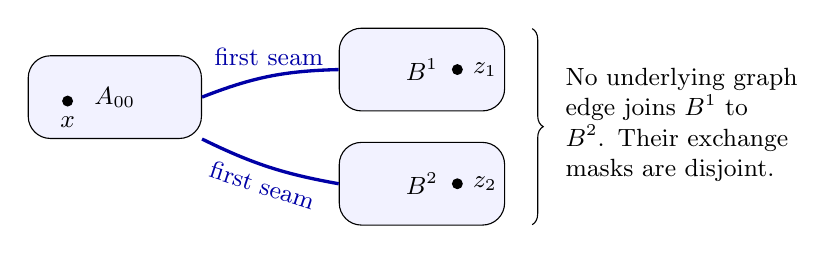
\begin{tikzpicture}[x=1cm,y=1cm,font=\small,
  piece/.style={draw,rounded corners=8pt,fill=blue!5,minimum width=1.65cm,minimum height=1.05cm},
  seam/.style={very thick,blue!65!black},dot/.style={circle,fill,inner sep=1.4pt}]
\node[piece,minimum width=2.2cm] (root) at (0.4,0) {$A_{00}$};
\node[piece,minimum width=2.1cm] (upper) at (4.3,.35) {$B^1$};
\node[piece,minimum width=2.1cm] (lower) at (4.3,-1.1) {$B^2$};
\draw[seam] (root.east) to[bend left=10] node[above] {first seam} (upper.west);
\draw[seam] (root.south east) to[bend right=8] node[below,sloped] {first seam} (lower.west);
\node[dot,label=below:$x$] at (-0.2,-.05) {};
\node[dot,label=right:$z_1$] at (4.75,.35) {};
\node[dot,label=right:$z_2$] at (4.75,-1.1) {};
\draw[decorate,decoration={brace,amplitude=4pt}] (5.7,.87)--(5.7,-1.62);
\node[align=left,anchor=west,text width=3cm] at (6,-.35)
{No underlying graph edge joins $B^1$ to $B^2$. Their exchange masks are disjoint.};
\end{tikzpicture}
\caption{Two hanging components in a common switched root cluster.
Undoing both insertions leaves $A_{00}$. Graph nonadjacency makes
the two collections of exchange masks disjoint. The proof recovers
each insertion from the jointly restored fields. The open seams
shown belong to the switched configuration; internal and other
incident edges are omitted.}
\label{fig:joint-inverse}
\end{figure}
